\documentclass{article}
\usepackage{fancyhdr}
\usepackage{ctex}
\usepackage{listings}
\usepackage{graphicx}
\usepackage[a4paper, body={18cm,22cm}]{geometry}
\usepackage{amsmath,amssymb,amstext,wasysym,enumerate,graphicx}
\usepackage{float,abstract,booktabs,indentfirst,amsmath}
\usepackage{array}
\usepackage{booktabs}
\usepackage{multirow}
\usepackage{url}
\usepackage{diagbox}
\renewcommand\arraystretch{1.4}
\usepackage{indentfirst}
\setlength{\parindent}{2em}
\usepackage{enumitem}
\setmonofont{Consolas}
\usepackage{listings}
\usepackage{xcolor}
\usepackage{makecell}
\usepackage{tikz}
\usetikzlibrary{positioning, arrows.meta}
\setCJKmonofont{黑体}
\lstset{  
	% 基本设置  
	xleftmargin = 3em, xrightmargin = 3em, aboveskip = 1em,  
	backgroundcolor = \color{white},  
	basicstyle = \small\ttfamily,  
	rulesepcolor = \color{gray},  
	breaklines = true,  
	numbers = left,  
	numberstyle = \small,  
	numbersep = -14pt,  
	frame = shadowbox,  
	showspaces = false,  
	columns = fixed,  
	sensitive = true,  
	% VSCode 风格配色  
	keywordstyle = \color{blue!70!black}\bfseries,  
	emphstyle = \color{red!70!black}\bfseries, % 对于强调的词  
	emphstyle=[2]\color{purple!70!black}\bfseries, % 对于第二组强调的词  
	commentstyle = \color{green!60!black}, % 注释颜色  
	stringstyle = \color{orange!90!black}, % 字符串颜色更亮一些  
	morekeywords={ASSERT, int64\_t, uint32\_t},  
	moreemph={ASSERT, NULL},  
	moreemph=[2]{int64\_t, uint32\_t, tid\_t, uint8\_t, int16\_t, uint16\_t, int32\_t, size\_t, bool},  
	morecomment=[l][\color{green!60!black}]{+}, % 以+开头的注释  
}

%--------------------页眉--------------------%
\pagestyle{fancy}
\fancyhead[L]{}
\fancyhead[R]{}
\fancyhead[C]{华东师范大学软件工程学院}
\fancyfoot[C]{-\thepage-}
\renewcommand{\headrulewidth}{1.5pt}
%--------------------标题--------------------%
\begin{document}
\begin{center}
	{\Large{\textbf{\heiti 第十二次作业——软件老化}}}
	\begin{table}[H]
		\centering
		\begin{tabular}{p{2cm}p{4cm}<{\centering}p{1cm}p{2cm}p{6cm}<{\centering}}
			课程名称:    & 软件质量分析 & \quad & 指导教师:    & 陈仪香
			\\ \cline{2-2} \cline{5-5}
			姓\qquad 名: & 王海生    & \quad & 学\qquad 号: & 10235101559
			\\ \cline{2-2} \cline{5-5}
			年\qquad 级: & 2023级    & \quad & 主\qquad 题: & 软件老化
			\\ \cline{2-2} \cline{5-5}
		\end{tabular}
	\end{table}
	
	% 添加新行并居中
	%\vspace{1em} % 可选:添加垂直间距
\end{center}
\rule{\textwidth}{1pt}

\tableofcontents

%--------------------正文--------------------%
\section{软件老化可信度量理论}

\subsection{可信计算框架}

为了评估软件系统随时间老化而降低其可信度,我们采用了一种称为可信计算框架的方法。该框架从研究软件老化相关的bug出发,通过提取失信证据、设计度量元,并根据这些度量元计算各个类别的可信度,最终汇总成一个综合的软件可信度量模型。

\begin{figure}[H]
	\centering
	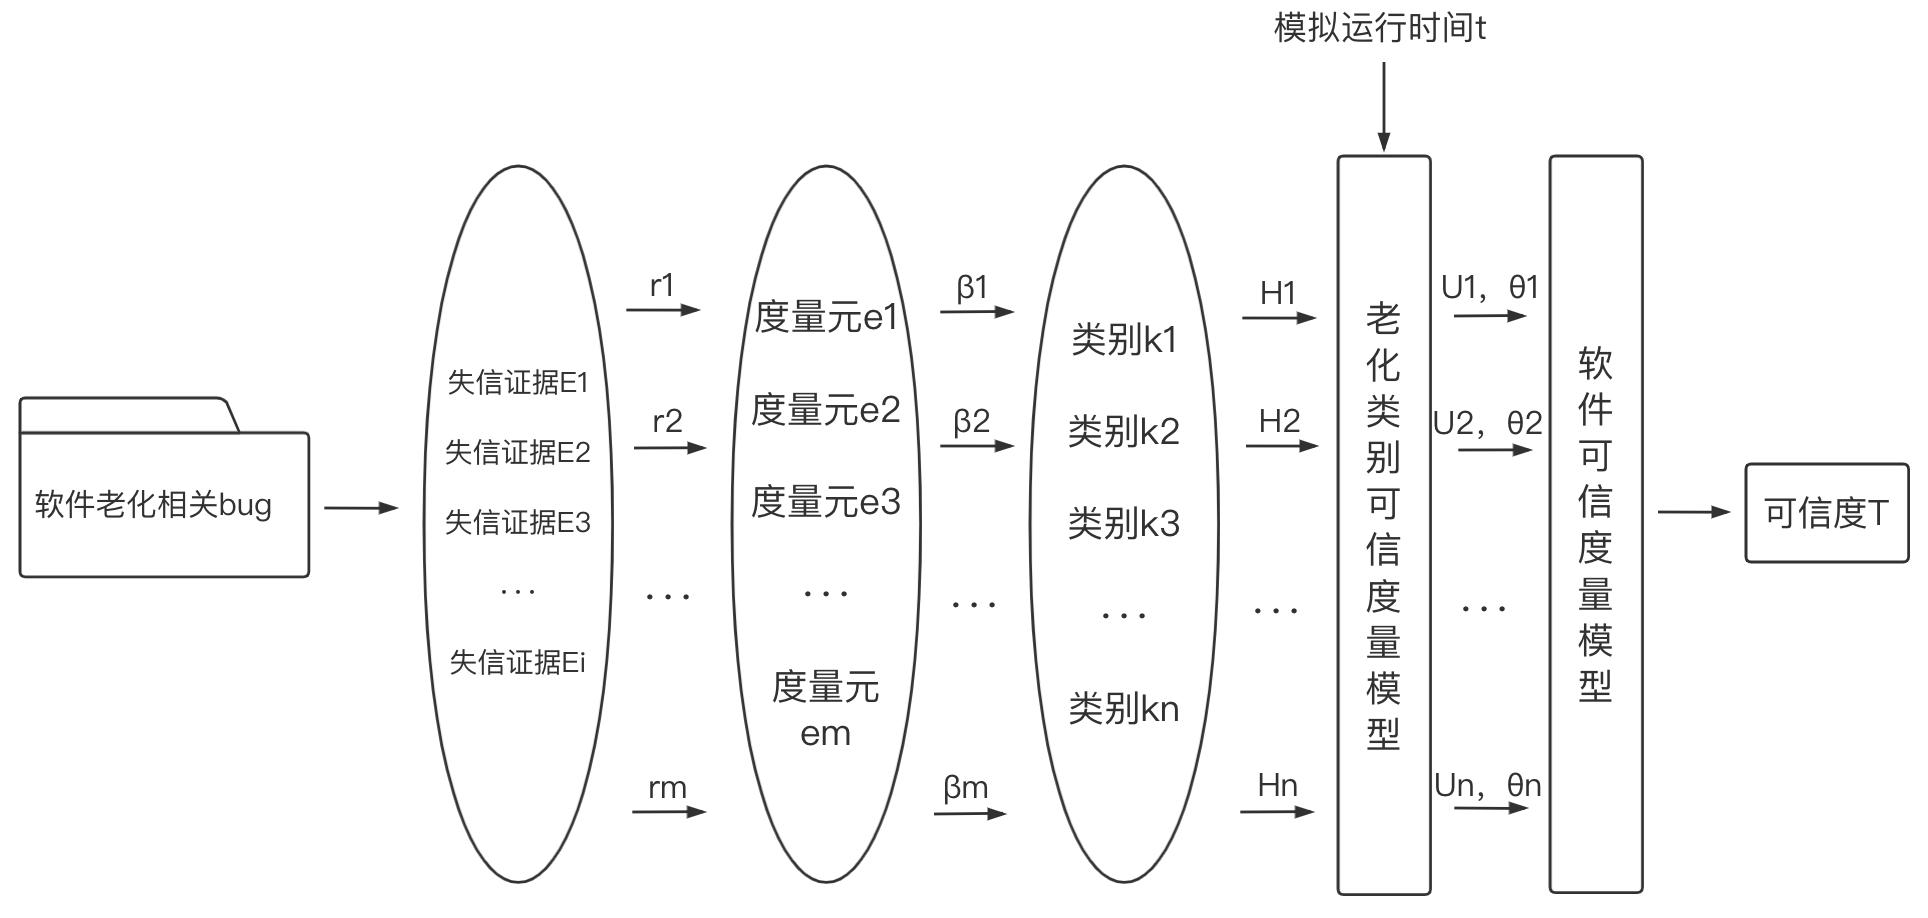
\includegraphics[width=0.9\textwidth]{img/1.png}
	\caption{可信计算框架}
\end{figure}

具体步骤如下:

\begin{enumerate}
	\item \textbf{提取失信证据}
	
	首先,从公共漏洞库中搜集与软件老化有关的bug报告。例如,在以下四个开源软件系统中收集了大量错误报告:
	\begin{itemize}
		\item Linux内核(Linux 2.6): \url{https://bugzilla.kernel.org}
		\item MySQL数据库管理系统(MySQL 5.1): \url{http://bugs.mysql.com}
		\item Apache HTTPD服务器(Apache HTTPD 2): \url{https://issues.apache.org/bugzilla}
		\item Apache AXIS框架: \url{https://issues.apache.org/jira/secure/IssueNavigator.jspa}
	\end{itemize}
	
	\item \textbf{设计度量元}
	
	基于上述失信证据,定义一系列度量元来量化不同类型的软件老化问题。每个度量元反映了特定的老化特征,比如内存泄漏、数值误差累积等。例如,针对浮点数寄存器误差和系统功能异常两个度量元(ARU类别),分别有1个实例(爱国者导弹事件)和3个实例(Linux3134, Linux5870, Linux7959)。
	
	\item \textbf{分类并计算各分类的可信度}
	
	将所有度量元按照导致软件老化的原因分成五个主要类别:MEM(内存管理)、STO(存储空间)、LOG(逻辑资源)、NUM(误差累积)及ARU(未知原因)。然后为每种类别计算其熵值$H_i(t)$,即该类别在时刻$t$的信息不确定性,以及对应的可信度$U_i(t)$。
	
	\item \textbf{度量元权重计算$\beta_i$}
	
	对于每一个度量元,我们需要确定它的相对重要性$\beta_i$。这可以通过比较同一类别内各个度量元的重要性来完成。例如,在ARU类别中,“浮点数寄存器误差”对应了一个实例,“系统功能异常”则对应了三个实例。因此,它们之间的权重分别为:
	$$
	\beta_1 = \frac{(1/3)}{(10/3)} = 0.10,\quad \beta_2 = \frac{(3)}{(10/3)} = 0.90
	$$
	
	\item \textbf{输入模拟运行时间,得到预期时间点的软件可信度}
	
	使用公式预测给定时间点$t$时软件的可信度$T(t)$。这里以某一具体类别为例,说明如何利用熵$H_i(t)$计算$K_i(t)$,进而获得整个系统的可信度$T(t)$。
	
	\item \textbf{汇总综合的软件可信度}
	
	最后,将所有类别的可信度加权求和,得到综合的软件可信度$T(t)$,其中$\theta_i$代表各类别的权重。公式如下:
	$$
	T(t) = \sum_{i=1}^{n} \theta_i \times U_i(t)
	$$
	其中,$U_i(t)$ 是第 $i$ 个类别在时刻 $t$ 的可信度,$\theta_i$ 是该类别的权重。
\end{enumerate}

通过以上步骤,我们可以建立一个完整的软件可信度计算框架,用以评估长期运行后的软件系统的可靠性和稳定性。

\subsection{度量元权重计算}

度量元权重计算是软件老化可信度量模型中的第一个重要环节,其目的是确定各个度量元在评估软件老化可信度时的相对重要程度。详细分析如下:

\begin{enumerate}
	\item \textbf{计算原理:}
	
	权重\(\beta_{i}\)代表了各度量元与同类型度量元相比的相对重要程度,数值越大说明该度量元对分类可信度的影响也就越大。通过每个度量元在统计数据中出现次数之比反应各度量元重要性的不同,该度量元对应的错误报告越多,说明该度量元对应的软件老化问题出现的越频繁,那这个度量元就越重要,对分类可信度的影响也就越大。
	
	\item \textbf{具体计算方法(以类别\(ARU\)为例):}
	
	\begin{enumerate}
		\item 类别\(ARU\)共有\(2\)个度量元:\(A1\)浮点数寄存器误差(\(1\)),\(A2\)系统功能异常(\(3\))。括号内数字表示该度量元包含的实例数目。
		\item 构造矩阵如下:
		\[
		\begin{array}{|c|c|c|c|c|}
			\hline
			& A1(1)\text{浮点数寄存器误差} & A2(3)\text{系统功能异常} & \text{行总计} & (\text{权重}i) \\
			\hline
			A1(1) &  & \frac{1}{3} & \frac{1}{3} & 0.10 \\
			\hline
			A2(3) & \frac{3}{1} &  & 3 & 0.90 \\
			\hline
			\text{列总计} & 3 & \frac{1}{3} & \frac{10}{3} &  \\
			\hline
		\end{array}
		\]
		\item 计算权重\(\beta_{1}\)和\(\beta_{2}\):
		\(\beta_{1}=\frac{\frac{1}{3}}{\frac{10}{3}} = 0.10\),\(\beta_{2}=\frac{3}{\frac{10}{3}} = 0.90\)
	\end{enumerate}
	
	\item \textbf{通用公式推导:}
	
	\begin{enumerate}
		\item 设类别\(k\)中有\(m\)个度量元,分别为\(e_{1},e_{2},\cdots,e_{m}\),其对应的实例数目分别为\(n_{1},n_{2},\cdots,n_{m}\)。
		\item 对于度量元\(e_{i}\),其在矩阵中的行总计为\(r_{i}=\sum_{j = 1}^{m}\frac{n_{i}}{n_{j}}\)(当\(i = j\)时,\(\frac{n_{i}}{n_{j}} = 1\))。
		\item 该类别所有行总计之和为\(R=\sum_{i = 1}^{m}r_{i}\)。
		\item 则度量元\(e_{i}\)的权重\(\beta_{i}=\frac{r_{i}}{R}\)。
	\end{enumerate}
	
	在实际计算中,对于不同的软件老化原因分类(如\(MEM\)、\(STO\)、\(LOG\)、\(NUM\)等),均按照上述方法分别计算其包含的度量元权重。例如,在类别\(LOG\)中,有\(7\)个度量元,通过类似的计算过程得出每个度量元的权重,如嵌套字功能异常\((\beta_{1}) = 0.2340\)、适配器选择错误\((\beta_{2}) = 0.1064\)等。这种计算方式能够合理地反映各个度量元在软件老化评估过程中的重要性差异,为后续的软件可信度计算提供重要依据。 
\end{enumerate}

\subsection{熵值计算}

度量元熵值计算是软件老化可信度量模型中的第二个重要环节,用于衡量软件运行状态的混乱程度。

\begin{enumerate}
	\item \textbf{度量元熵值的定义与计算原理:}
	
	基于软件老化的失信证据度量元的熵是在单一该度量元影响下,表示软件运行状态混乱程度的量。其考虑了预期内运行状态和风险状态,因为风险状态越多软件运行偏离预期的可能性越大,系统越混乱,熵就会增大。熵值计算公式为$$ S = \log_{10} r(t) $$其中\(r(t)\)为度量元对应的最大风险值。由于度量元可能有两个风险值,这里取最大风险值进行计算。例如在一些实际案例中,像 Linux 的某些缺陷导致的度量元,其风险值可根据具体的软件占用资源情况、对系统性能影响时间等因素确定,进而通过该公式计算出熵值。
	
	\item \textbf{类别熵值的计算方法:}
	
	软件老化原因分类的熵是在由同一种软件老化原因导致的基于软件老化的失信证据度量元影响下,衡量软件运行状态混乱程度的量,且是软件运行时间的函数。其计算公式为$$ H(t)=\sum_{i = 1}^{n}\beta_{i}\log_{10}r_{i}(t) $$其中\(\beta_{i}\)为第\(i\)个度量元的权重(采用 Brassard 的计算方式),\(r_{i}(t)\)为第\(i\)个度量元的最大风险值。以 MEM 类别为例,如果有多个与内存管理相关的度量元,如内存需求过大、内存泄漏等,先确定每个度量元的权重\(\beta_{i}\)和最大风险值\(r_{i}(t)\),然后按照公式计算该类别在时刻\(t\)的熵值。单一类型的熵值越高,代表该类型度量元可能引发软件老化的风险越大,软件可信度随时间降低的速度也就越快。
\end{enumerate}

\subsection{类别可信度计算}

类别可信度计算是软件老化可信度量模型中的第三个重要环节,用于评估不同软件老化原因类别对软件可信度的影响。其具体计算过程为:

\begin{enumerate}
	\item 设计得到老化类别可信度量模型,各类别可信度与时间\(t\)的关系函数为$$ K_{i}(t)=e^{-H_{i}(t)} $$其中\(K_{i}(t)\)为第\(i\)个类别在时刻\(t\)的可信度,\(H_{i}(t)\)为第\(i\)个软件老化类别在时刻\(t\)的熵,\(t\)为软件运行时间。
	
	\item 
	为了优化可信度的值域,将各类别\(i\)可信度对软件可信度分类可信度的值域\([0,1]\)进行调整,采用十分制,值域为\([1,10]\)。因此\(i\)类别可信度的十分制表示为$$ U_{i}(t)=\left\{\begin{array}{c}10e^{-H_{i}(t)}, 0.1\leq e^{-H_{i}(t)}\leq 1 \\ 1, 0\leq e^{-H_{i}(t)}<0.1\end{array}\right.$$
\end{enumerate}

\subsection{软件可信度计算}

软件可信度计算是软件老化可信度量模型中的最后一个重要环节,其模型为:

\[
T(t)=\begin{cases}
	\prod_{i = 1}^{n}U_{i}(t)^{\theta_{i}},&1\leq U_{i}(t)\leq10\\
	\sum_{i = 1}^{n}\theta_{i}=1,&0\leq\theta_{i}\leq1
\end{cases}
\]

在此公式中,\(\theta_{i}(i = 1,\cdots,n)\)代表各类别的权重,这些权重反映了不同类别在软件可信度评估体系中的相对重要程度。通过将各类别经过前面一系列计算所得到的可信度\(U_{i}(t)\),按照其对应的权重\(\theta_{i}\)进行幂运算后连乘(当\(1\leq U_{i}(t)\leq10\)时),或者在满足权重和为\(1\)且\(0\leq\theta_{i}\leq1\)的条件下进行相关运算,最终实现将各分类可信度汇总整合,从而得出软件在时刻\(t\)的综合可信度\(T(t)\)。 

\section{编程计算软件可信属性}

\subsection{题目}

编程或使用课程提供的Python代码,实现下列功能:

\begin{itemize}
	\item \textbf{输入:}类别,以及类别中每个度量元的含例子个数。
	\item \textbf{输出:}在时刻\texttt{t = 0}和\texttt{t = 10}情况下,四个类别的熵和可信度,以及软件可信度.
\end{itemize}

已知的可信属性如下图所示:

\begin{figure}[H]
	\centering
	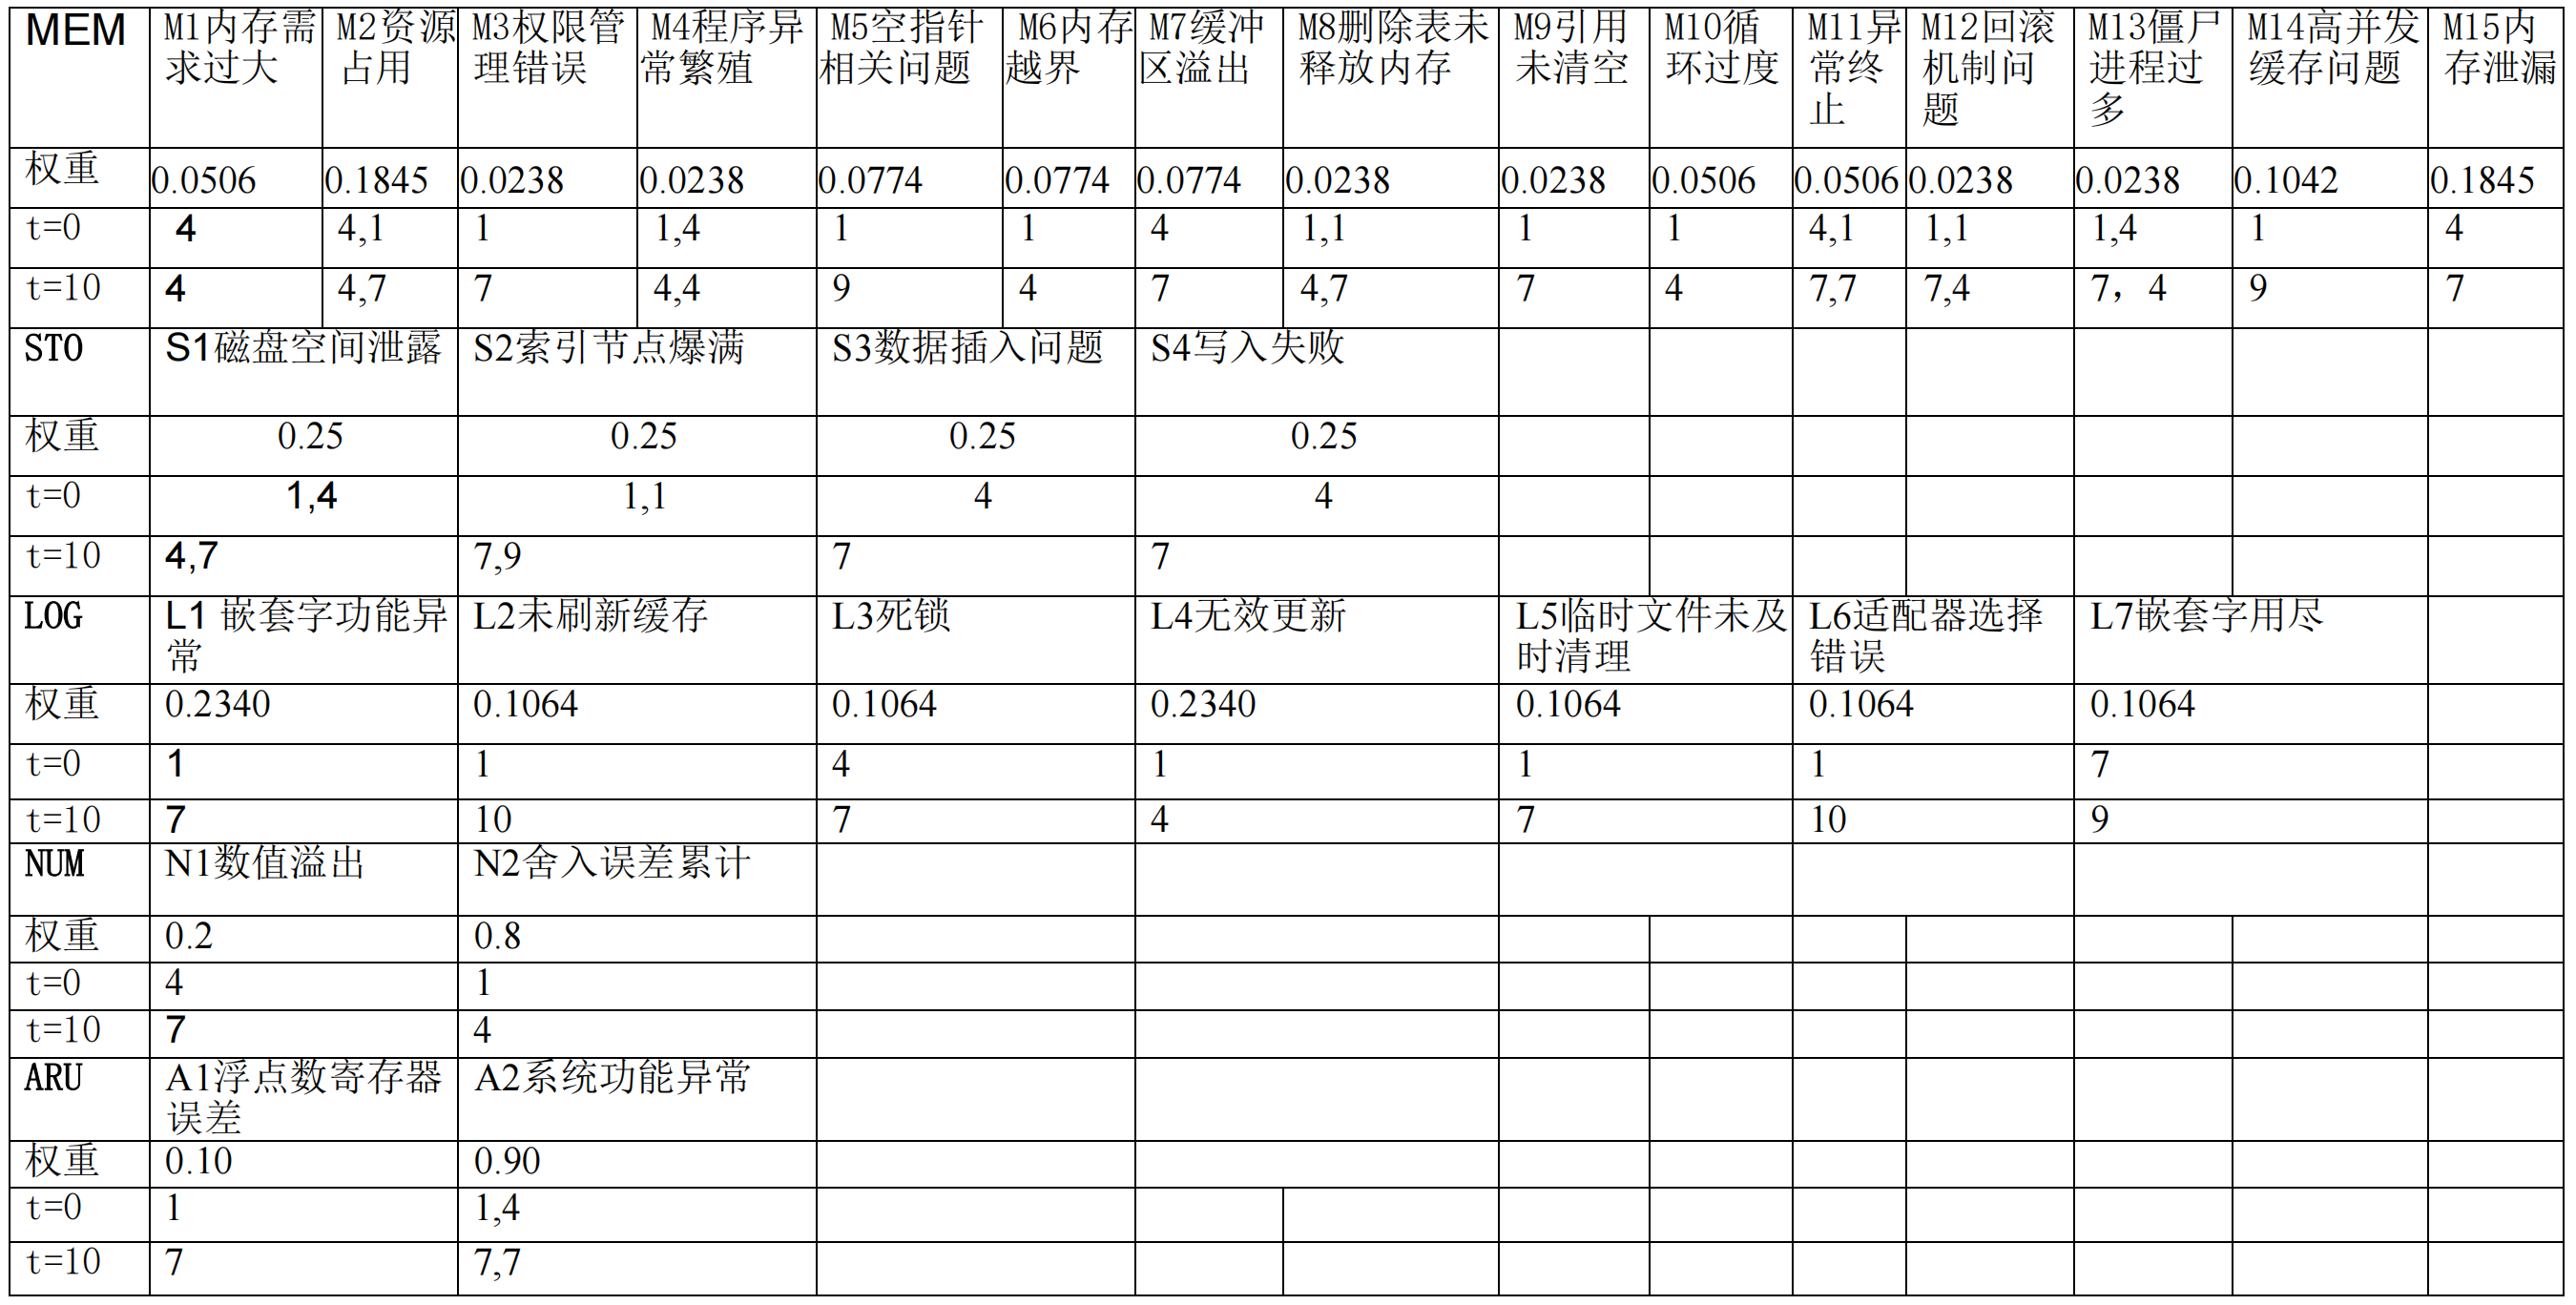
\includegraphics[width=0.9\textwidth]{img/2.png}
	\caption{已知可信属性}
\end{figure}

\subsection{代码}

根据软件老化可信度量模型,编写\texttt{Python}代码如下:

\begin{lstlisting}[language=Python]
	import math
	
	n = int(input("类别数:"))
	
	theta = []
	theta_str = input("各个类别的权重:").split(" ")
	for t in theta_str:
	theta.append(float(t))
	
	m = []
	m_str = input("各个类别的度量元数量:").split(" ")
	for num in m_str:
	m.append(int(num))
	
	R = [] # 存储权重和最大风险
	BETA = []
	
	for i in range(n):
	beta = []
	beta_str = input("第{0}个类别-各个度量元的权重:".format(i + 1)).split(" ")
	for b in beta_str:
	beta.append(float(b))
	BETA.append(beta)
	
	r = []
	r_str = input("第{0}个类别-各个度量元的该时刻最大风险值:".format(i + 1)).split(" ")
	for value in r_str:
	r.append(float(value))
	R.append(r)
	
	Hs = [] # 熵
	Us = [] # 类别可信值
	
	for i in range(n):
	H = 0
	for j in range(m[i]):
	H += BETA[i][j] * math.log10(R[i][j])
	U = max(10 * math.exp(-H), 1)
	Hs.append(H)
	Us.append(U)
	
	print("各类别的熵:{0}".format(Hs))
	print("各类别的可信值:{0}".format(Us))
	
	T = 1
	for i in range(n):
	T *= math.pow(Us[i], theta[i])
	print("可信值:{0}".format(T))
	
\end{lstlisting}

\subsection{结果}

当\texttt{t = 0}时,代码运行结果如下图所示:

\begin{figure}[H]
	\centering
	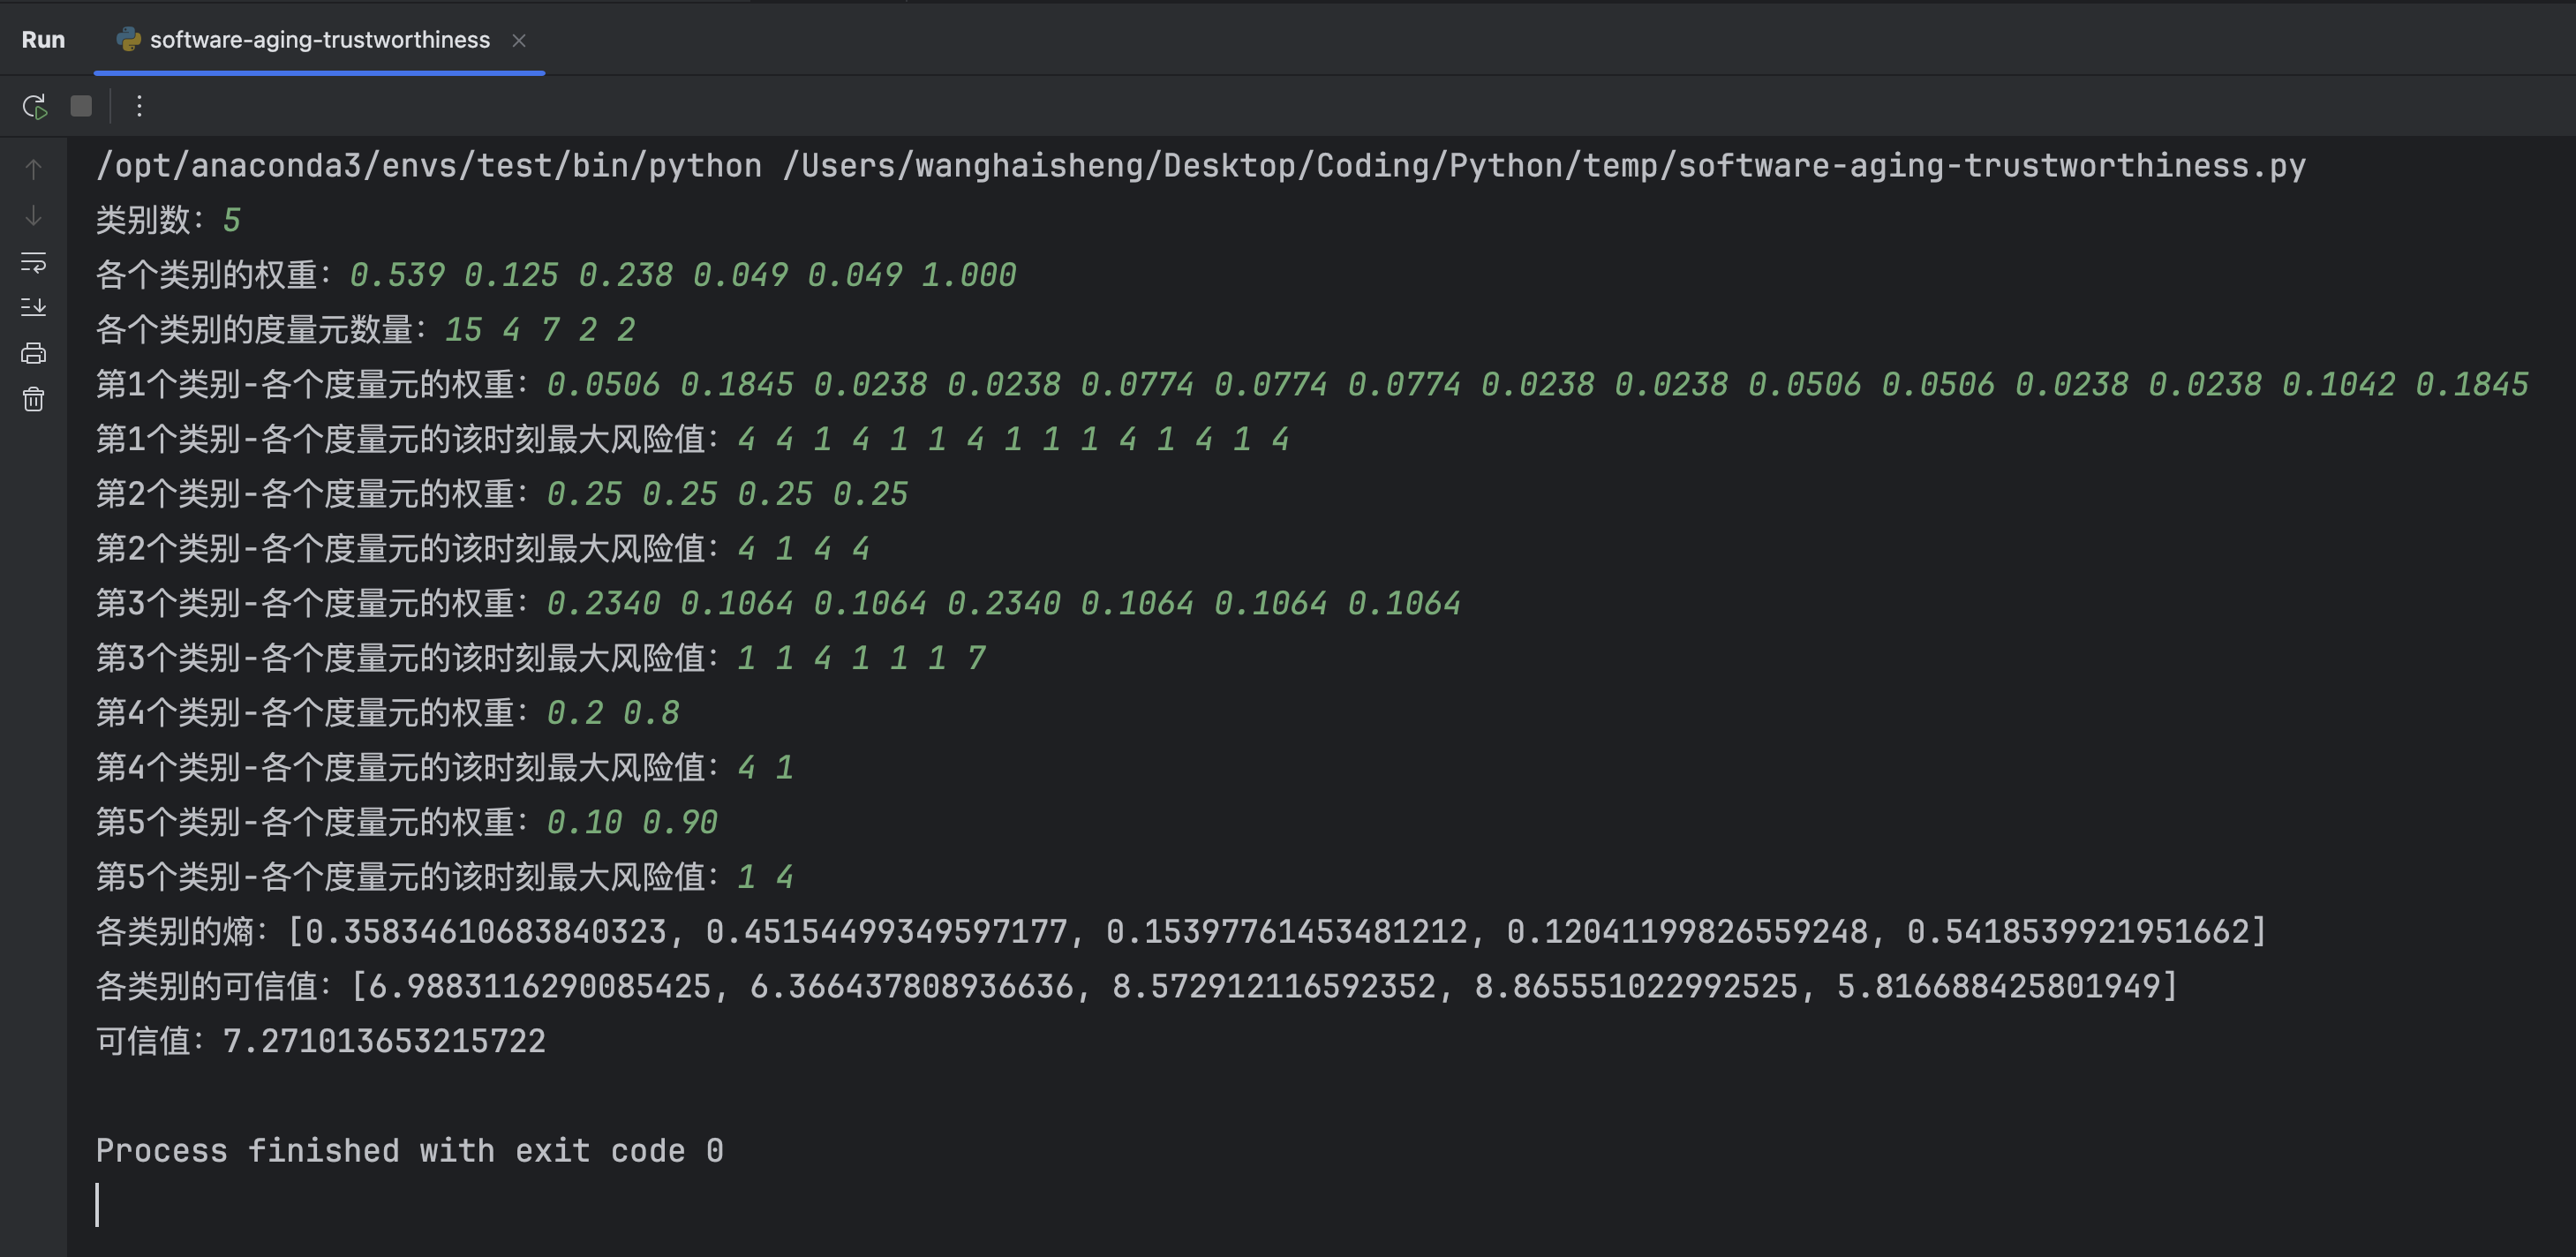
\includegraphics[width=0.9\textwidth]{img/3.png}
	\caption{\texttt{t = 0}运行结果}
\end{figure}

当\texttt{t = 10}时,代码运行结果如下图所示:

\begin{figure}[H]
	\centering
	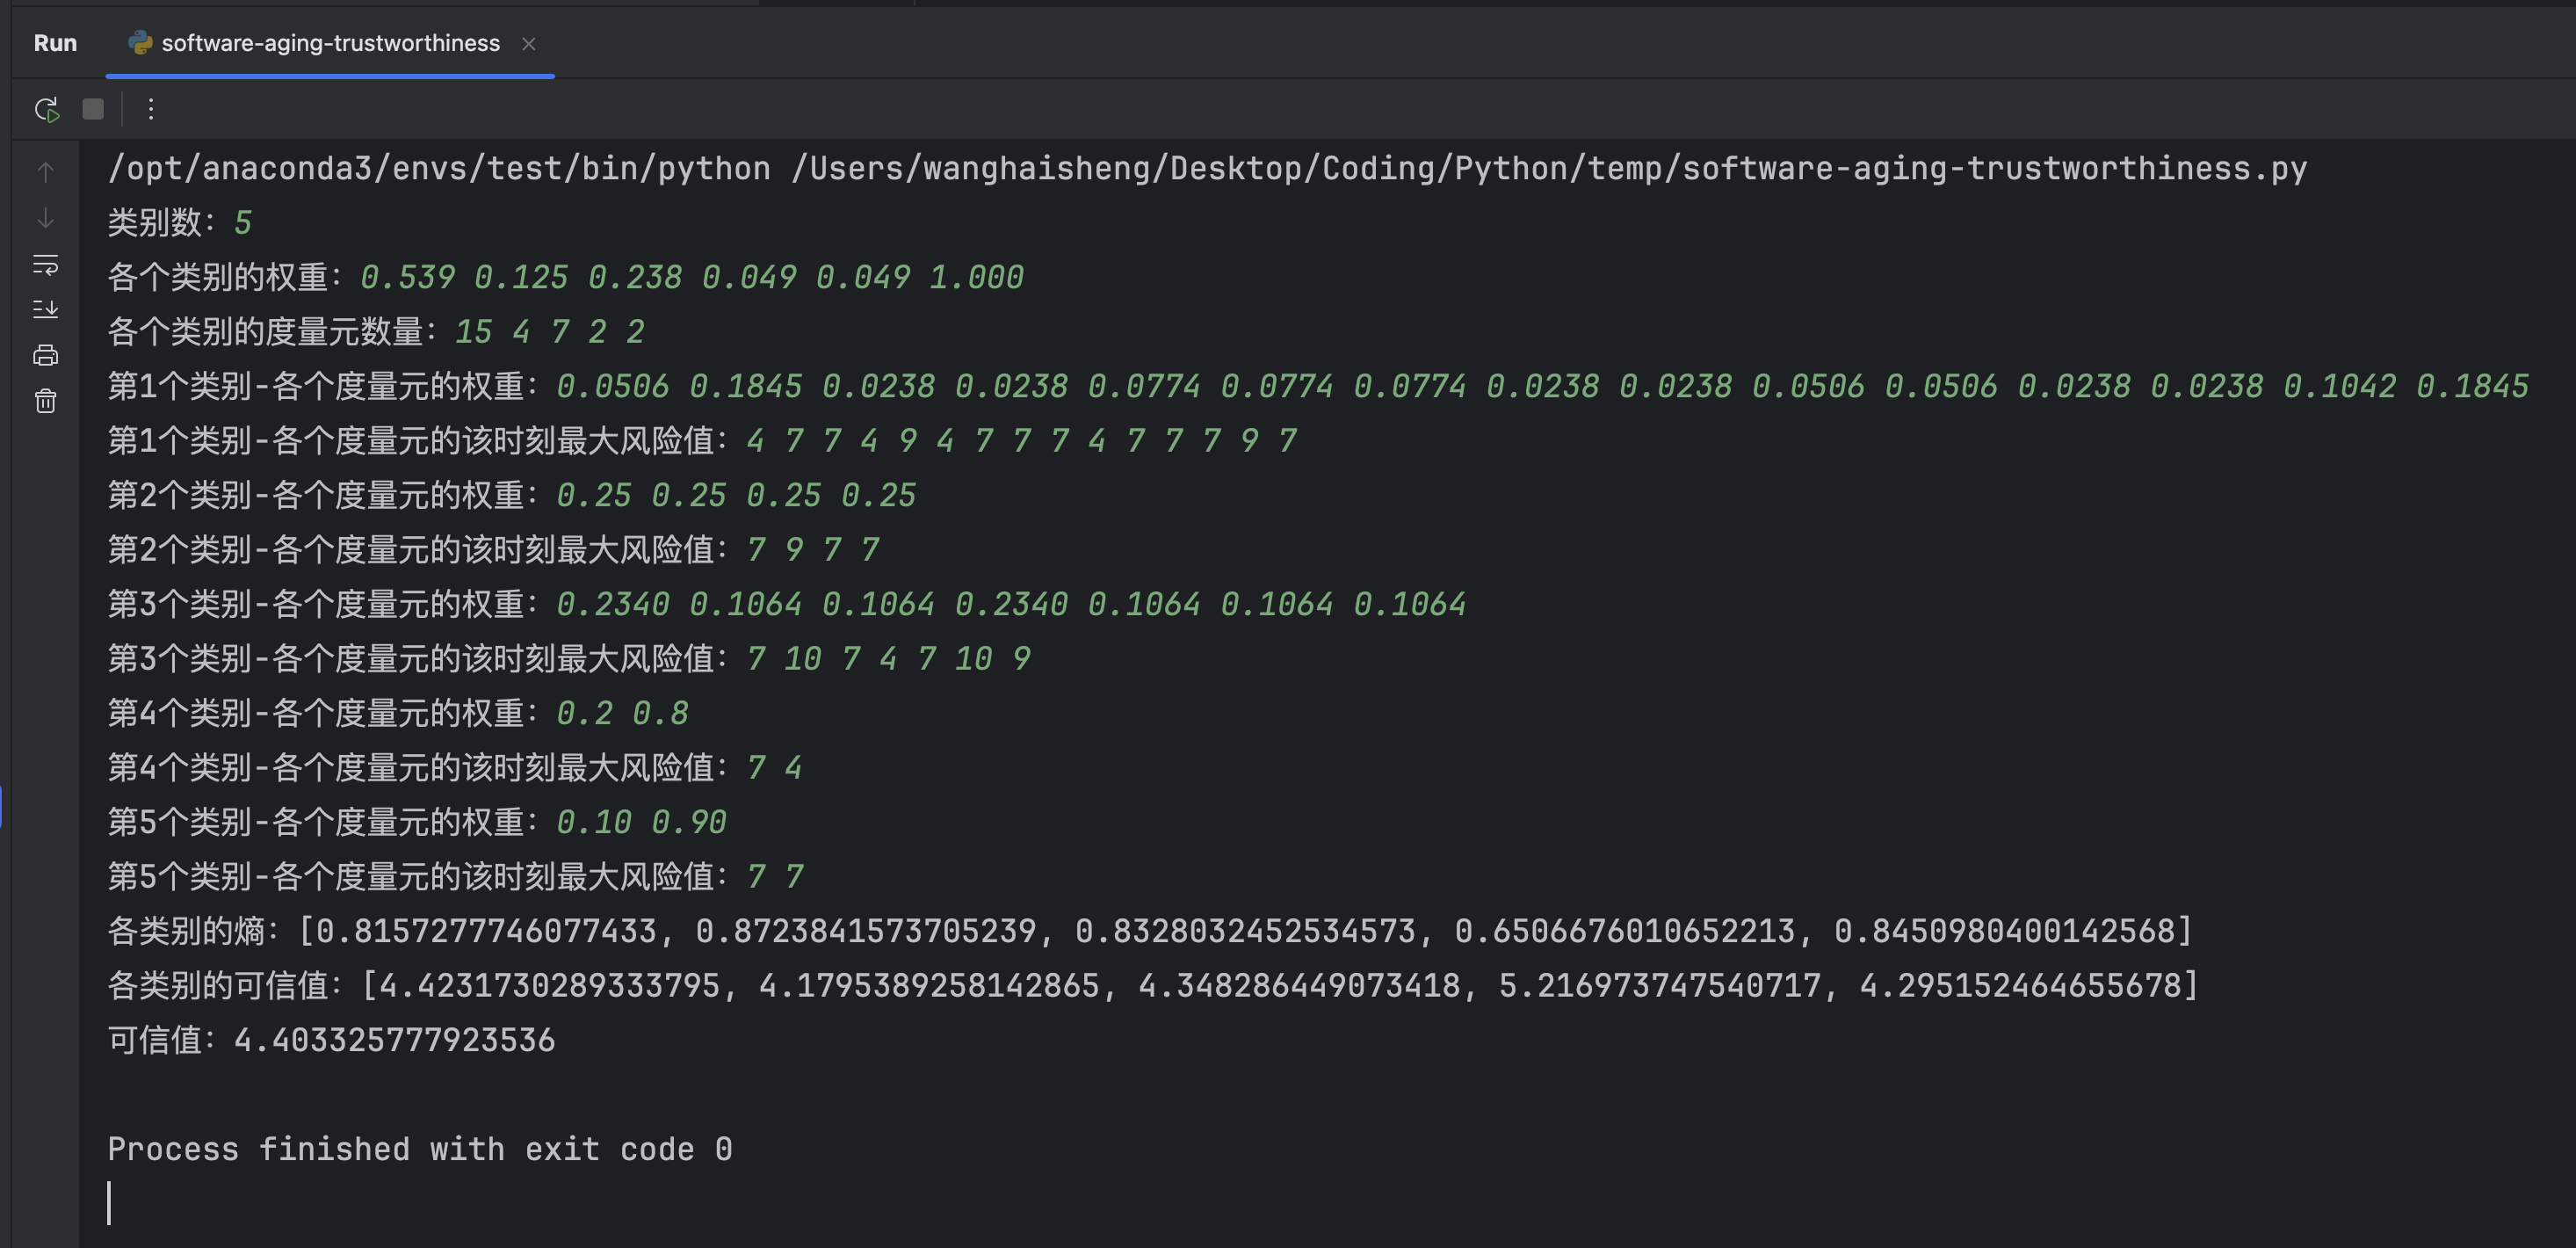
\includegraphics[width=0.9\textwidth]{img/4.png}
	\caption{\texttt{t = 10}运行结果}
\end{figure}

由此可得,四个类别的熵和可信度如下表所示:

\begin{center}
	\begin{tabular}{|c|c|c|c|c|c|c|}
		\hline
		& 时间 & MEM & STO & LOG & NUM & ARU \\
		\hline
		熵 & t=0 & 0.358 & 0.452 & 0.154 & 0.120 & 0.542 \\
		\cline{2-7}
		& t=10 & 0.816 & 0.872 & 0.833 & 0.651 & 0.845 \\
		\hline
		可信度 & t=0 & 6.988 & 6.366 & 8.573 & 8.866 & 5.817 \\
		\cline{2-7}
		& t=10 & 4.423 & 4.180 & 4.348 & 5.217 & 4.295 \\
		\hline
	\end{tabular}
\end{center}

可信度如下表所示:

\begin{center}
	\begin{tabular}{|c|c|}
		\hline
		时间 & 软件可信度 \\
		\hline
		t=0 & 7.271 \\
		\hline
		t=10 & 4.403 \\
		\hline
	\end{tabular}
\end{center}

\end{document}